%%%%%%%%%%%%%%%%%%%%%%%%%%%%%%%%%%%%%%%%%%%%%%%%%%%%%%%%%%%
% --------------------------------------------------------
% Tau
% LaTeX Template
% Version 2.4.4 (28/02/2025)
%
% Author: 
% Guillermo Jimenez (memo.notess1@gmail.com)
% 
% License:
% Creative Commons CC BY 4.0
% --------------------------------------------------------
%%%%%%%%%%%%%%%%%%%%%%%%%%%%%%%%%%%%%%%%%%%%%%%%%%%%%%%%%%%

\documentclass[9pt,a4paper,twocolumn,twoside]{tau-class/tau}
\usepackage[english]{babel}

\usepackage{array}      % For column formatting
\usepackage{booktabs}   % Professional table lines
\usepackage{lipsum}     % For dummy text (optional)
%\usepackage{array} % For better column formatting
\usepackage{booktabs} % For professional-looking tables
\usepackage{stfloats}     % Better float handling in two-column
\usepackage{enumitem}     % Customize itemize
\usepackage{adjustbox}    % Scale table if needed

% Compact itemize for tables
\newenvironment{tabitemize}{%
  \begin{itemize}[leftmargin=*,nosep,itemsep=-2pt,topsep=0pt]
}{%
  \end{itemize}
}


%% Spanish babel recomendation
% \usepackage[spanish,es-nodecimaldot,es-noindentfirst]{babel} 

%% Draft watermark
% \usepackage{draftwatermark}

%----------------------------------------------------------
% TITLE
%----------------------------------------------------------

\journalname{Policy Paper}
\title{Positioning the PALM and RSE schemes in Tonga 2024}

%----------------------------------------------------------
% AUTHORS, AFFILIATIONS AND PROFESSOR
%----------------------------------------------------------

\author[a,1]{Antonio Moeaki}
\author[a,2]{Etina Tuipulotu}
\author[a,3]{Manu Fukofuka}

%----------------------------------------------------------

\affil[a]{EFPD Economists}
%\affil[b]{Senior Economist}
%\affil[c]{Principal Economist}

\professor{Ministry of Finance, Tonga}

%----------------------------------------------------------
% FOOTER INFORMATION
%----------------------------------------------------------

%\institution{\LaTeX\ Template}
\footinfo{Ministry of Finance, Tonga}
\theday{May 26, 2025}
\leadauthor{Ministry of Finance}
\course{Economic and Fiscal Policy Division}

%----------------------------------------------------------
% ABSTRACT AND KEYWORDS
%----------------------------------------------------------

\begin{abstract}    
    Tonga's participation in labor mobility schemes (PALM and RSE) has generated substantial economic and social benefits for Tonga, including increased remittances, skills transfer, and poverty reduction. However, the displacement of a large number of local workers overseas has led to emerging issues such as labor shortages, overdependence on the scheme and family issues that raise concerns about the long-term sustainability of these programs. This paper critically examines the trends of the PALM and RSE schemes on Tonga’s labor market. It is found that PALM intake for Tonga is dropping, with a shift in preference for long-term contracts; whilst RSE is growing sustainably and offers insight on the need for a more equitable rotation of seasonal workers. Features such as remittance dependency, insights on worker productivity, and policy responses are scrutinized to form a policy recommendation that can strengthen the structural challenges facing Tonga's future economic development. 
    
    
    
    %whether the benefits of overseas employment outweigh its structural challenges for Tonga’s development.
\end{abstract}

%----------------------------------------------------------

\keywords{Labour Mobility Sceheme, PALM, RSE, Remittances, Tonga}

%----------------------------------------------------------

\begin{document}
		
    \maketitle 
    \thispagestyle{firststyle} 
    \tauabstract 
    % \tableofcontents
    % \linenumbers 
    
%----------------------------------------------------------

\section{Introduction}

    \taustart{T}onga has participated in labor mobility schemes since 2007, including New Zealand's Recognised Seasonal Employer (RSE) scheme, Australia’s Seasonal Worker Programme (SWP) and the Pacific Labour Scheme (PLS) introduced in 2018. By 2022, the SWP and PLS programs were merged into a single program - introducing the Pacific Australia Labor Mobility (PALM) scheme. These programs have shaped Tonga's socio-economic landscape - generating 59.2 million (U.S dollars) for Tonga in 2024 - primarily through the expansion of employment opportunities available to the working-age population. The target beneficiaries - often rural workers with few formal job prospects - can now gain access to seasonable employment abroad ranging across 5 industry groups: Agriculture, Meat Processing, Accommodation, Health and Social Assistance, and other industries - over short-term (up to 9 months) or long-term contracts (4 years). As a result, we are seeing a boost in household incomes and a facilitation of the transfer of skills from returning seasonal workers bringing valuable human capital back to Tonga. The results of these programmes have - therefore - become an invaluable component of Tonga's long-term prosperity. %strategy.

    %Labour mobility is one of the primary economic opportunities available to the working-age population in the region, with the potential to generate significant economic and social benefits for workers (e.g. financial income, work experience and skills development including formal qualifications); their home countries (e.g. unemployment relief, development of human and financial capital, reduction in finance trade deficits and investment in community assets); and Australia (e.g. alleviation of labour shortages, increased production and greater competitiveness). A ‘triple win’
    

\section{Why should we be concerned?}

    As of 2022-23, 11.4\% of Tonga's working age population (goes up to 20.4\% for males) participate in the Australia and New Zealand labor mobility scheme - one of the highest amongst Pacific countries. It is reported that more than 25\% of households in Tonga declare remittances as their \textbf{main} source of income - highlighting the vitality of these programs to the livelihood of Tonga (HIES, 2021) \cite{HIES}. Clearly, Tonga shows a profound economic dependence on these schemes. Beyond the immediate benefits, these programs have complex social dimensions that create issues such as: workforce gaps in local industries, a high-remittance dependent country, systemic gaps in skills and training, and stress on 6 family relationships. 
    
    The following are noted:

   \textbf{Local workforce shortages} - 
   The number of government vacancies has doubled from 2022-2025 due to increasing exits from government work.

	        \begin{table}[H]
            \centering
            \caption{Government Vacancies}
            \label{tab:table}
            \begin{tabular}{lllll}
                \toprule
                \textbf{Object} & \textbf{2022}& \textbf{2023}& \textbf{2024} & \textbf{2025}
                \\
                \midrule
                Vacancies & 496 & 597 & 759 & 861 \\
                \bottomrule     
            \end{tabular}
			
            \tabletext{Source: \cite{Budget_Statement} Ministry of Finacne}
			
        \end{table}
 The key drivers of these vacancies are \\ \textbf{(i)} Higher compensation available for technical positions on donor funded projects \\ \textbf{(ii)} Migration. \\
 \textbf{(iii)} An outflow of skilled workers on these labor schemes. In the past year, 392 \textit{skilled } workers left on seasonal work - 7\% of the current vacancies coming from government workers. Given this small statistic of government workers, this draws greater attention to the other pressing issue of the labor shortage: mismatch of skills from education to the workplace.
 
  % Within that number, 56\% are between Most of these Tongans in these mobility schemes are medium or unskilled workers.  \\

   	%Fig. \ref{fig:figure} shows the \textit{total} number of Tongan workers in Australia.
    		
    		
    	\begin{figure}[H]
    		\centering
    		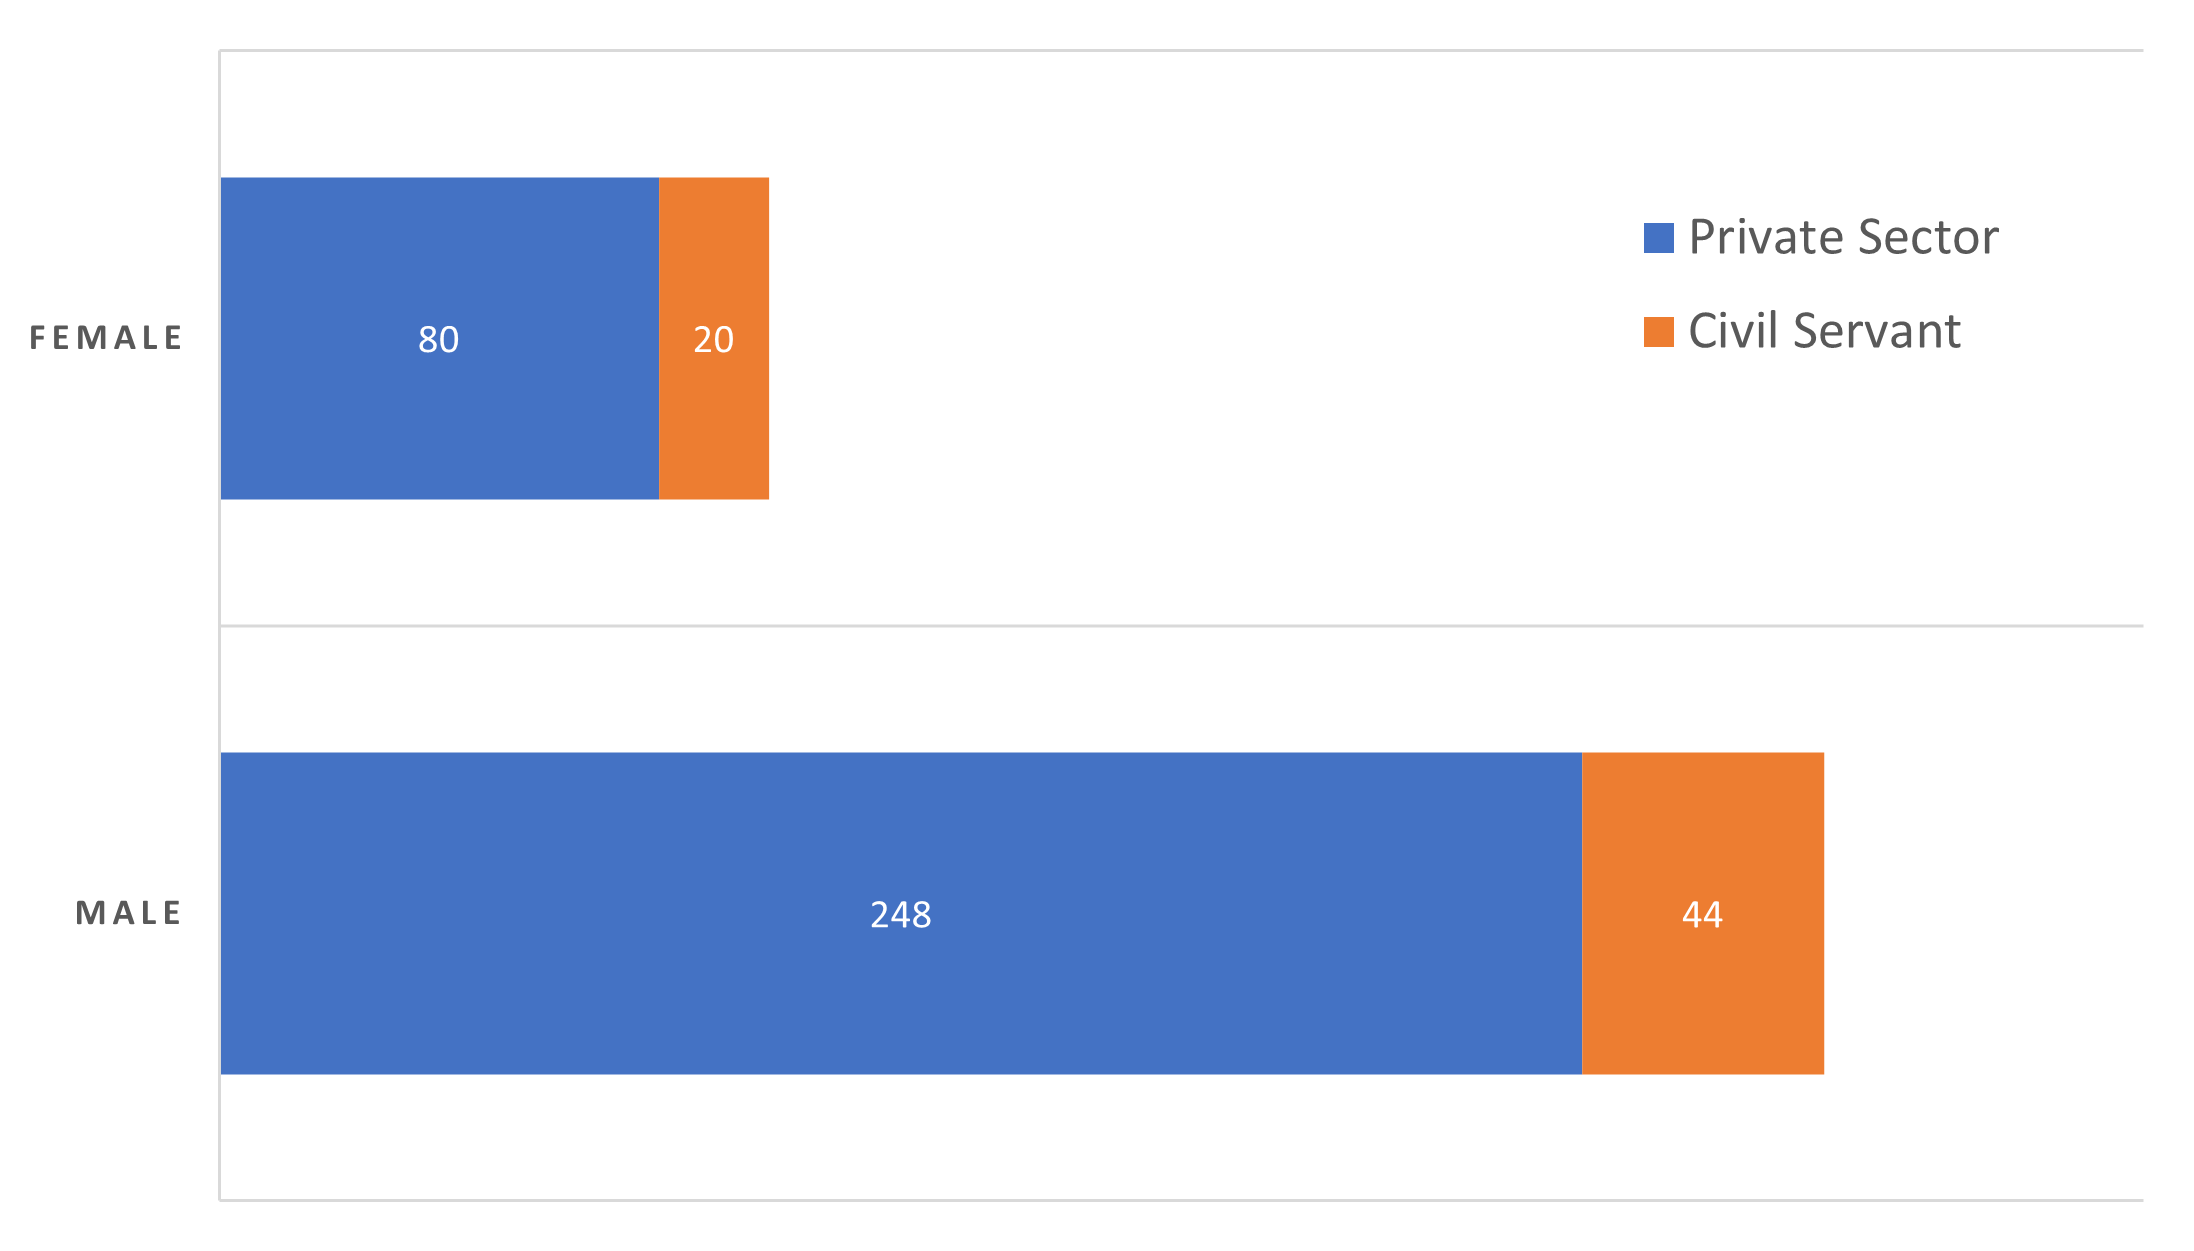
\includegraphics[width=0.9\columnwidth]{figures/Civil_data.png}
    		\caption{Skilled workers leaving on labor mobility schemes}
    		\label{fig:figure}
    	\end{figure}

   
   %According to the HIES 2021, over 25\% of households in Tonga have remittances as their main source of income (HIES, 2021). Talk about workforce shortages - eg local farmers due to people leaving on mobility schemes resulted in farm product prices going up due to higher unit costs. Puloka pointed out that government projects have been delayed due to local labourers travelling overseas to participate in these schemes.


\textbf{Mismatch of skills and educational outcomes} - Nested within the labor drain, as identified by the \textit{Skills and Employment for Tongans} (SET) project, are the systemic gaps in education and skills development within Tonga which do not supply the skills demanded by domestic and international job markets. Job creation was also limited, with majority coming mostly from the public sector. From the labor-demand side, employers are reporting difficulties in finding staff with appropriate skills  (foundational, socio-emotional and technical) and report a lack of recognition for Tonga's national certifications.  Hence, reforms to improve educational outcomes for job readiness will combat both the trends of the outflow via labor migration and the fill-ins of local vacancies. 

%For the poorest households, barriers to education start as early as school-age, with less than three among five children not attending secondary schools due to financial constraints, lack of motivation for academic pursuits and a notion that schools did not meet the supply of skills required for the workplace. 

\textbf{Overdependence on scheme} - Inadvertently, the schemes have entrenched Tonga in a cycle of dependency—both for individuals and the broader economy. In 2025, Tonga's high remmittance dependency (42.4\% of GDP) makes the economy vulnerable to exogenous shocks such as regulatory changes in Australia, exchange rate volatility and global exposing the nation’s economic precarity. As a result, internal structural issues such as a lack of diversified job opportunities and a workforce conditioned to see overseas labor as their only viable livelihood.

%For Tonga to achieve long-term economic resilience, seasonal work must evolve from a temporary survival strategy into a stepping stone for skill development and entrepreneurship. Many returning workers possess valuable experience in agriculture, construction, and logistics—skills that could be repurposed to boost Tonga’s domestic economy. However, without targeted training, access to capital, or incentives to invest in local businesses, workers often re-enter the same cycle, repeatedly migrating for short-term contracts.






   \textbf{Effect on local families} - An important adverse effect of labor schemes is it's fragmentation of families in the Pacific, reflected through prolonged parental absence, disrupted gender roles, increased marital instability and lasting psychological harm to children and communities. The WCCC highlights 57 new family issue cases in Tonga that relate to labor mobility schemes which requires government intervention and support that isn't necessarily available.

   %The nature of these schemes being male-dominated disturbs child development and imposes a dual burden on women to be both breadwinners and caregivers in a family setting.
	
\section{Analysis}

    The trend of remittances - and the local dependence on it -  is an important component for labor schemes in Tonga. In the past 3 years, the breakdown of remittance components (\textit{Compensation of overseas workers \& Personal remittances}) rose from 35.3 to 62.3 and 180.6 to 211.9 respectively as shown below: 

    	        \begin{table}[H]
            \centering
            \caption{Tonga's Remittances (millions U.S. Dollars)}
            \label{tab:table}
            \begin{tabular}{lll}
                \toprule
                \textbf{Object} & \textbf{2022} & \textbf{2024}
                \\
                \midrule
                Remittances & 215.9 & 257.6 \\
                \hspace{5mm} \textit{\% of GDP} & 45.4 & 42.4 \\
                \hspace{5mm} \textit{Compensation of overseas workers} & 35.3 & 59.2 \\
               \hspace{5mm}  \textit{Personal remittances} & 180.6 & 203.9 \\
               %\midrule
               \cline{2-3}
               PALM & 6035 & 3040 \\
               RSE & 987 & 1307 \\
                \bottomrule     
            \end{tabular}
			
            \tabletext{Source: \cite{IMF_ArticleIV} IMF Article IV 2024}
			
        \end{table}

        Despite the overall fall of seasonal workers (\textit{due to the drop in PALM workers}), remittances via overseas workers (\$ 59.2m) are trending upwards driven by the persistence of long-term contracts (which are multiplicatively more valuable than short-term contracts). The bigger pool of remittances (\$203.9 m) from permanent migrants is strengthened by economic recovery of destination countries which increases diaspora income, exchange rate value and improved remittance channels. \\
        The following sections will consider PALM and RSE separately and in greater detail:

       % \newpage
        
\section{Pacific Australia Labor Mobility (PALM)}

	\begin{tauenv}[frametitle=Background]
  For the year 2024, PALM provided seasonal work to more than 30,000 employees from the Pacific and Timor-Leste (as of Novermber). On average, workers are remitting an average of A\$1061-1300 monthly and generate almost \$1 billion in industry value added per year. The Australian Government has committed \$440 million across successive budgets to help expand the program -  i.e to help PALM workers complete certifications, allowing for family to come with LT workers, and making seasonal deployments more attractive by reducing the burden of upfront of travel costs.
                 	\end{tauenv}





PALM's sources from 10 countries across the Pacific and Timor-Leste - including Fiji, Kiribati, Nauru, Papua New Guinea, Samoa, Solomon Island, Timor-Leste, Tuvalu, Vanuatu and \textbf{Tonga}. 
		
    	Fig. \ref{fig:TotalPALM} shows the \textit{total} number of Tongan workers in Australia..
    		
    	\begin{figure}[H]
    		\centering
    		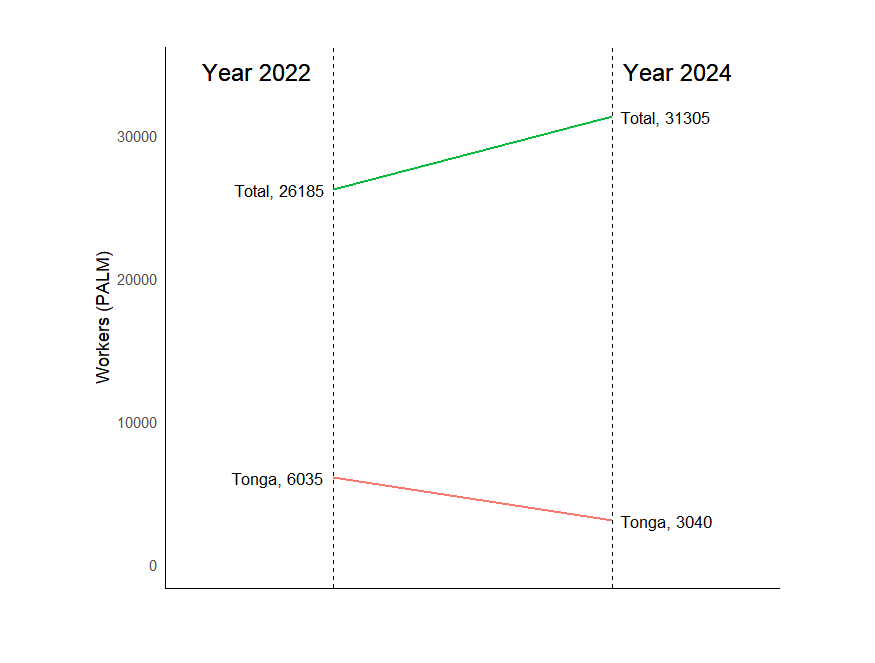
\includegraphics[width=.9\columnwidth]{figures/TongaPALM.png}
    		\caption{The scheme has grown between 2022-2025}
    		\label{fig:TotalPALM}
    	\end{figure}
		
        %Fig. \ref{fig:examplefloat} shows an example of two figures that covers the width of the page. It can be placed at the top or bottom of the page. The space between the figures can also be changed using the \verb|\hspace{Xpt}| command.
		
    %    \begin{figure*}[bp] % t for position at the top of the current page; b for position at the bottom; p for new page
%		\centering
%		  \begin{subfigure}[b]{0.38\linewidth} % Fig (a)
			%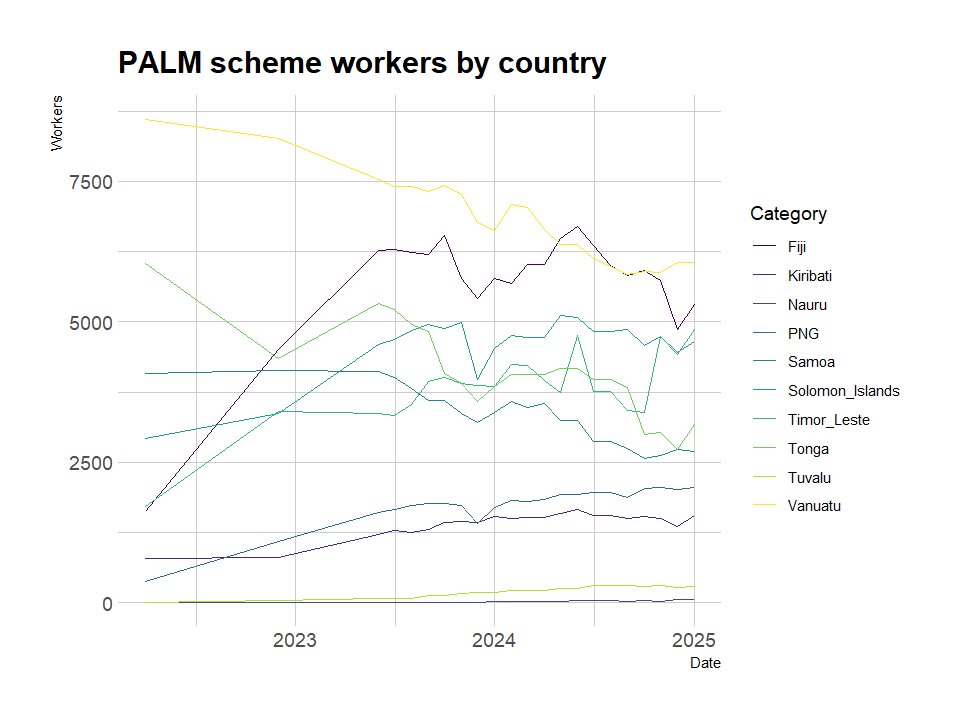
\includegraphics[width=\linewidth]{figures/PALM_country.png}
		%	\caption{Breakdown by country}
		%	\label{fig:figa}
		%\end{subfigure}
		%	\hspace{20pt}   % Space between the figures
		%\begin{subfigure}[b]{0.375\linewidth} % Fig (b)
			%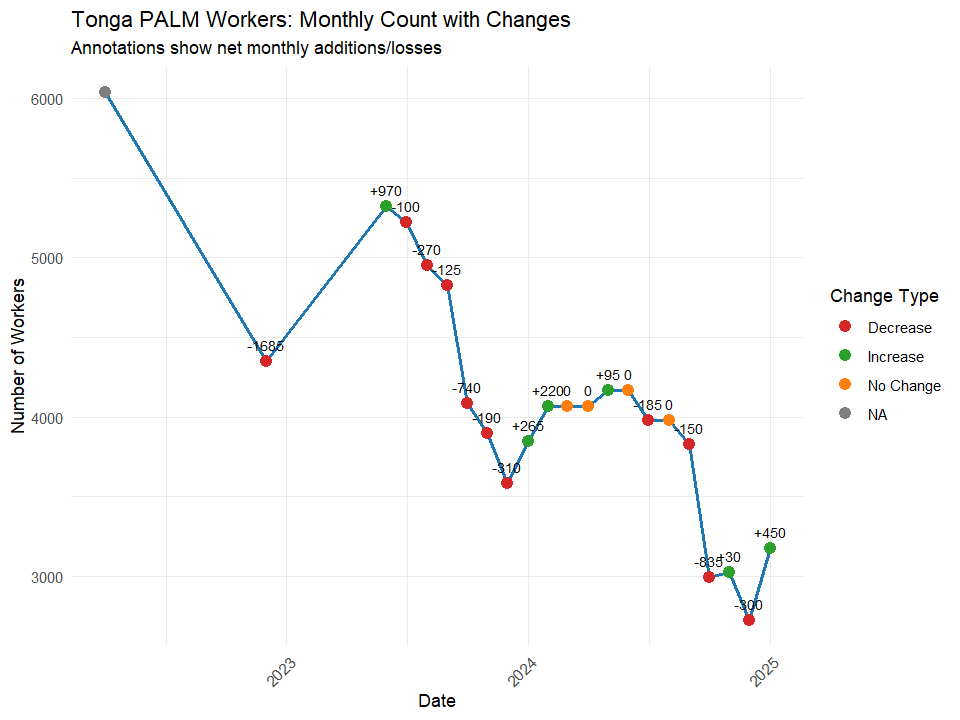
\includegraphics[width=\linewidth]{figures/Monthly changes.png}
		%	\caption{Tonga's monthly changes.}
		%	\label{fig:figb}
		%\end{subfigure}
		%\caption{Tonga's falling PALM intake \cite{PFGPlots}.}
		%\label{fig:examplefloat}
	%\end{figure*}

     Notably, by 2024 the total PALM workers from Tonga has halved (down to 3,040) since 2022 amidst the growing size of the PALM scheme (from 26,185 to 1,305) as of 2024. The key reasons identified for this falling number of workers from Tonga are:

     \begin{enumerate}
  
 
  \item The value of short-term vs long-term contracts
   \item Alternative seasonal workers (Backpackers)
 % \item Misuse of scheme
\end{enumerate}

%Stiffer Rules → Higher Compliance Costs → Short-Term Contracts Become Unprofitable → Employers Opt for Long-Term Roles → Tonga’s Seasonal Workers Face Fewer Opportunities  

    \subsection{Short-term vs Long-term contracts} Tonga's PALM intake is dominated by short-term contracts accounting for 67\% of the total Tongan workers. These roles mainly refer to agricultural fruitpicking and harvesting roles.
    It appears that for countries with pre-dominantly short-term seasonal roles (such as Tonga (67\%), Samoa (54\%), and Vanuatu (84\%))- they appear to suffer a drop in the total intake of PALM workers due to the revised Deed of agreement issued in June 2023. 
     
  
    
    
    

    	Fig. \ref{fig:PALMCOUNTRY} plots PALM workers trends by country
    		
    		
    	\begin{figure}[H]
    		\centering
    		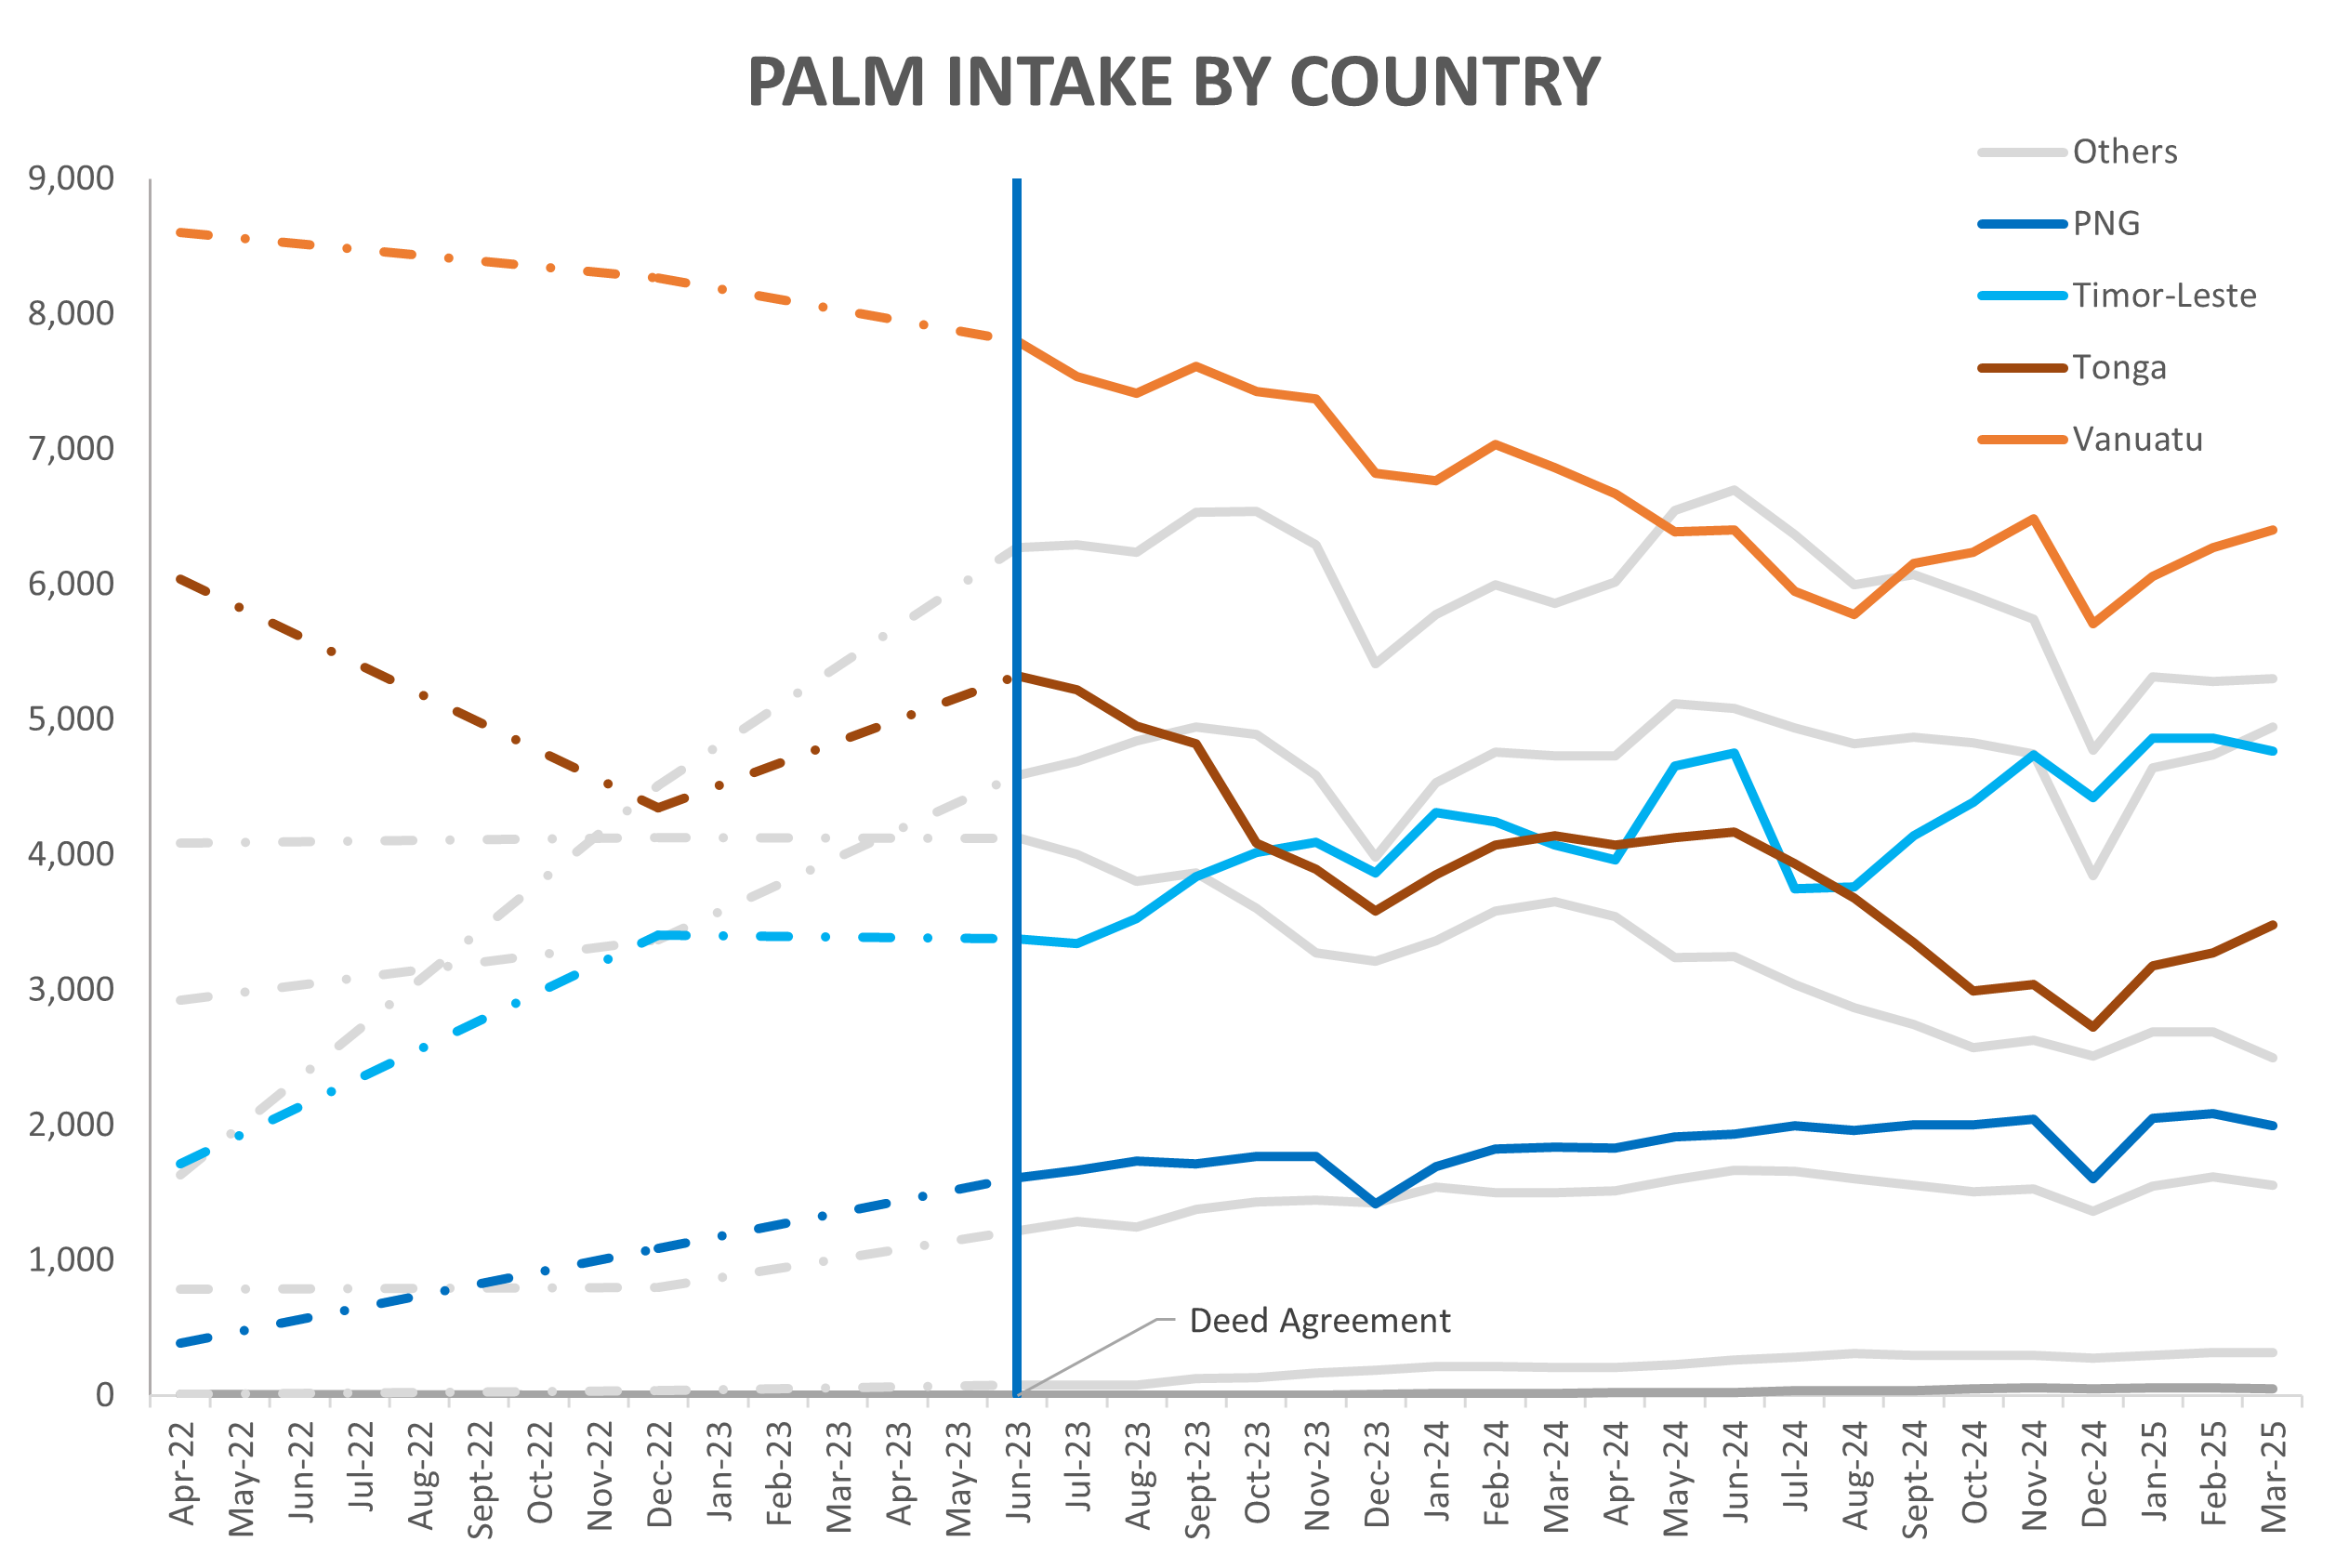
\includegraphics[width=0.9\columnwidth]{figures/CountryPALMFINAL.png}
    		\caption{Post Deed of Agreement favors long-term contracts}
    		\label{fig:PALMCOUNTRY}
    	\end{figure}

 The June 2023 deed of agreement strengthened protection for Pacific workers by mandating minimum weekly pay gurantees, regulated hours, improved accommodation standards, and compulsory trainings - all which increase the burden on approved employers. While these reforms successfully curb worker exploitation, they also raised compliance costs for employers leading to two key outcomes.

  \begin{itemize}
   \item \textbf{Decline in employers} - Due to the higher burden of compliance, employers have either decided to withdraw from the program entirely or are pushed towards hiring backpackers. SWP employers reported an expected reduction in demand for short-term PALM workers of between 17 to 25 per cent \cite{Bradford},to manage the new financial risk and loss of flexibility.
   \\


  
        	Fig. \ref{fig:shortvslong} shows the \textit{total} number of Tongan workers in Australia.
    		
    		
    	\begin{figure}[H]
    		\centering
    		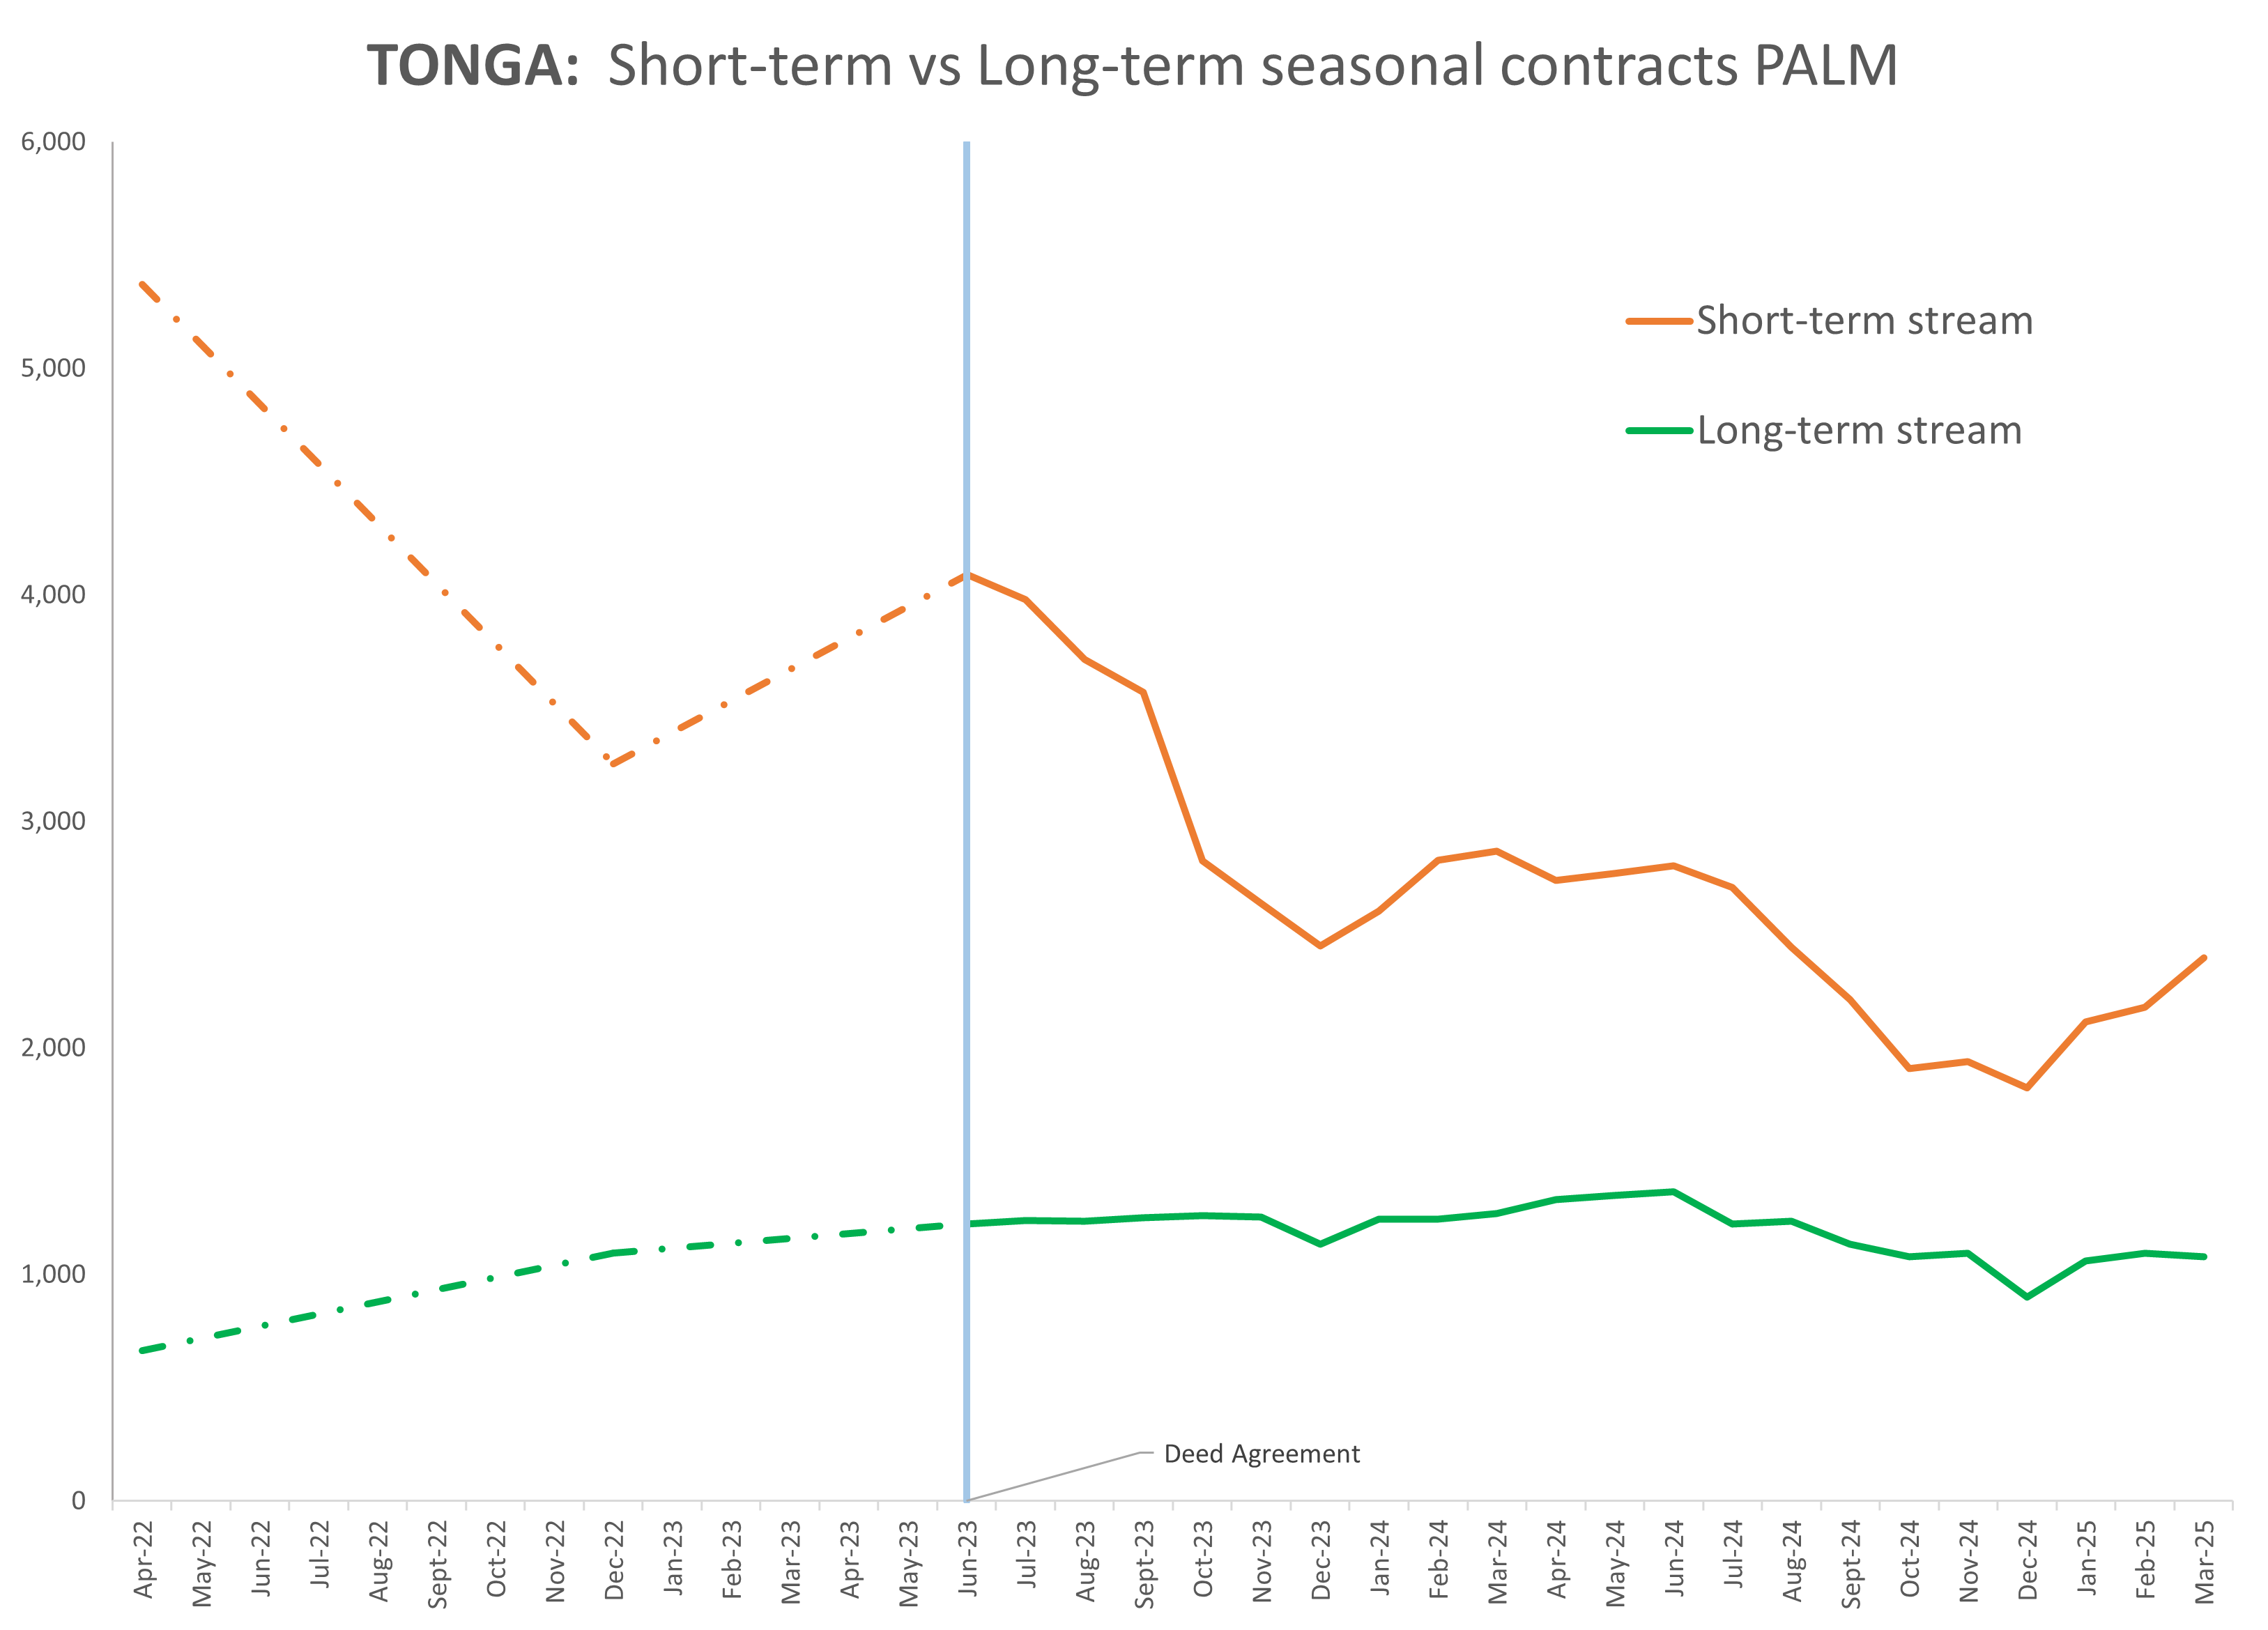
\includegraphics[width=0.9\columnwidth]{figures/Tonga_short-term.png}
    		\caption{Post Deed of Agreement favors long-term contracts}
    		\label{fig:shortvslong}
    	\end{figure}

          \item \textbf{Decline in Short-term contracts} - these roles became less viable due to higher fixed costs (employers had to gurantee 120 paid hours over four weeks and provide year-round accommodation even for 6month short term roles \cite{Bradford_a}
          
\end{itemize}

 
 
 %brought stricter protection laws for seasonal workers through improved contract terms concerning minimum weekly pay, hours of work, accommodation, and training of workers - preventing exploitation of workers. \textbf{This} resulted in higher compliance costs for employers - making short-term contracts unprofitable and shifted the preference towards long-term roles - causing the drop in overall PALM workers. However, the value of these long-term contracts (which is steadily rising) offsets the drop in short-term roles allowing the flow of remittances to retain its momentum.

 







	%\begin{equation} \label{ec:equation}
%	Remittances = \beta_0 + \beta_1 *PALM + \beta_2*RSE + \epsilon
%	\end{equation} 


\subsection{Competition from destination country}

Working holiday maker (WHM) visa holders, more commonly known as backpackers, are the main alternative source of labour for growers because they handle their own travel and accommodation costs - being less expensive for employers.



	%\begin{figure}[H]
    %		\centering
    %		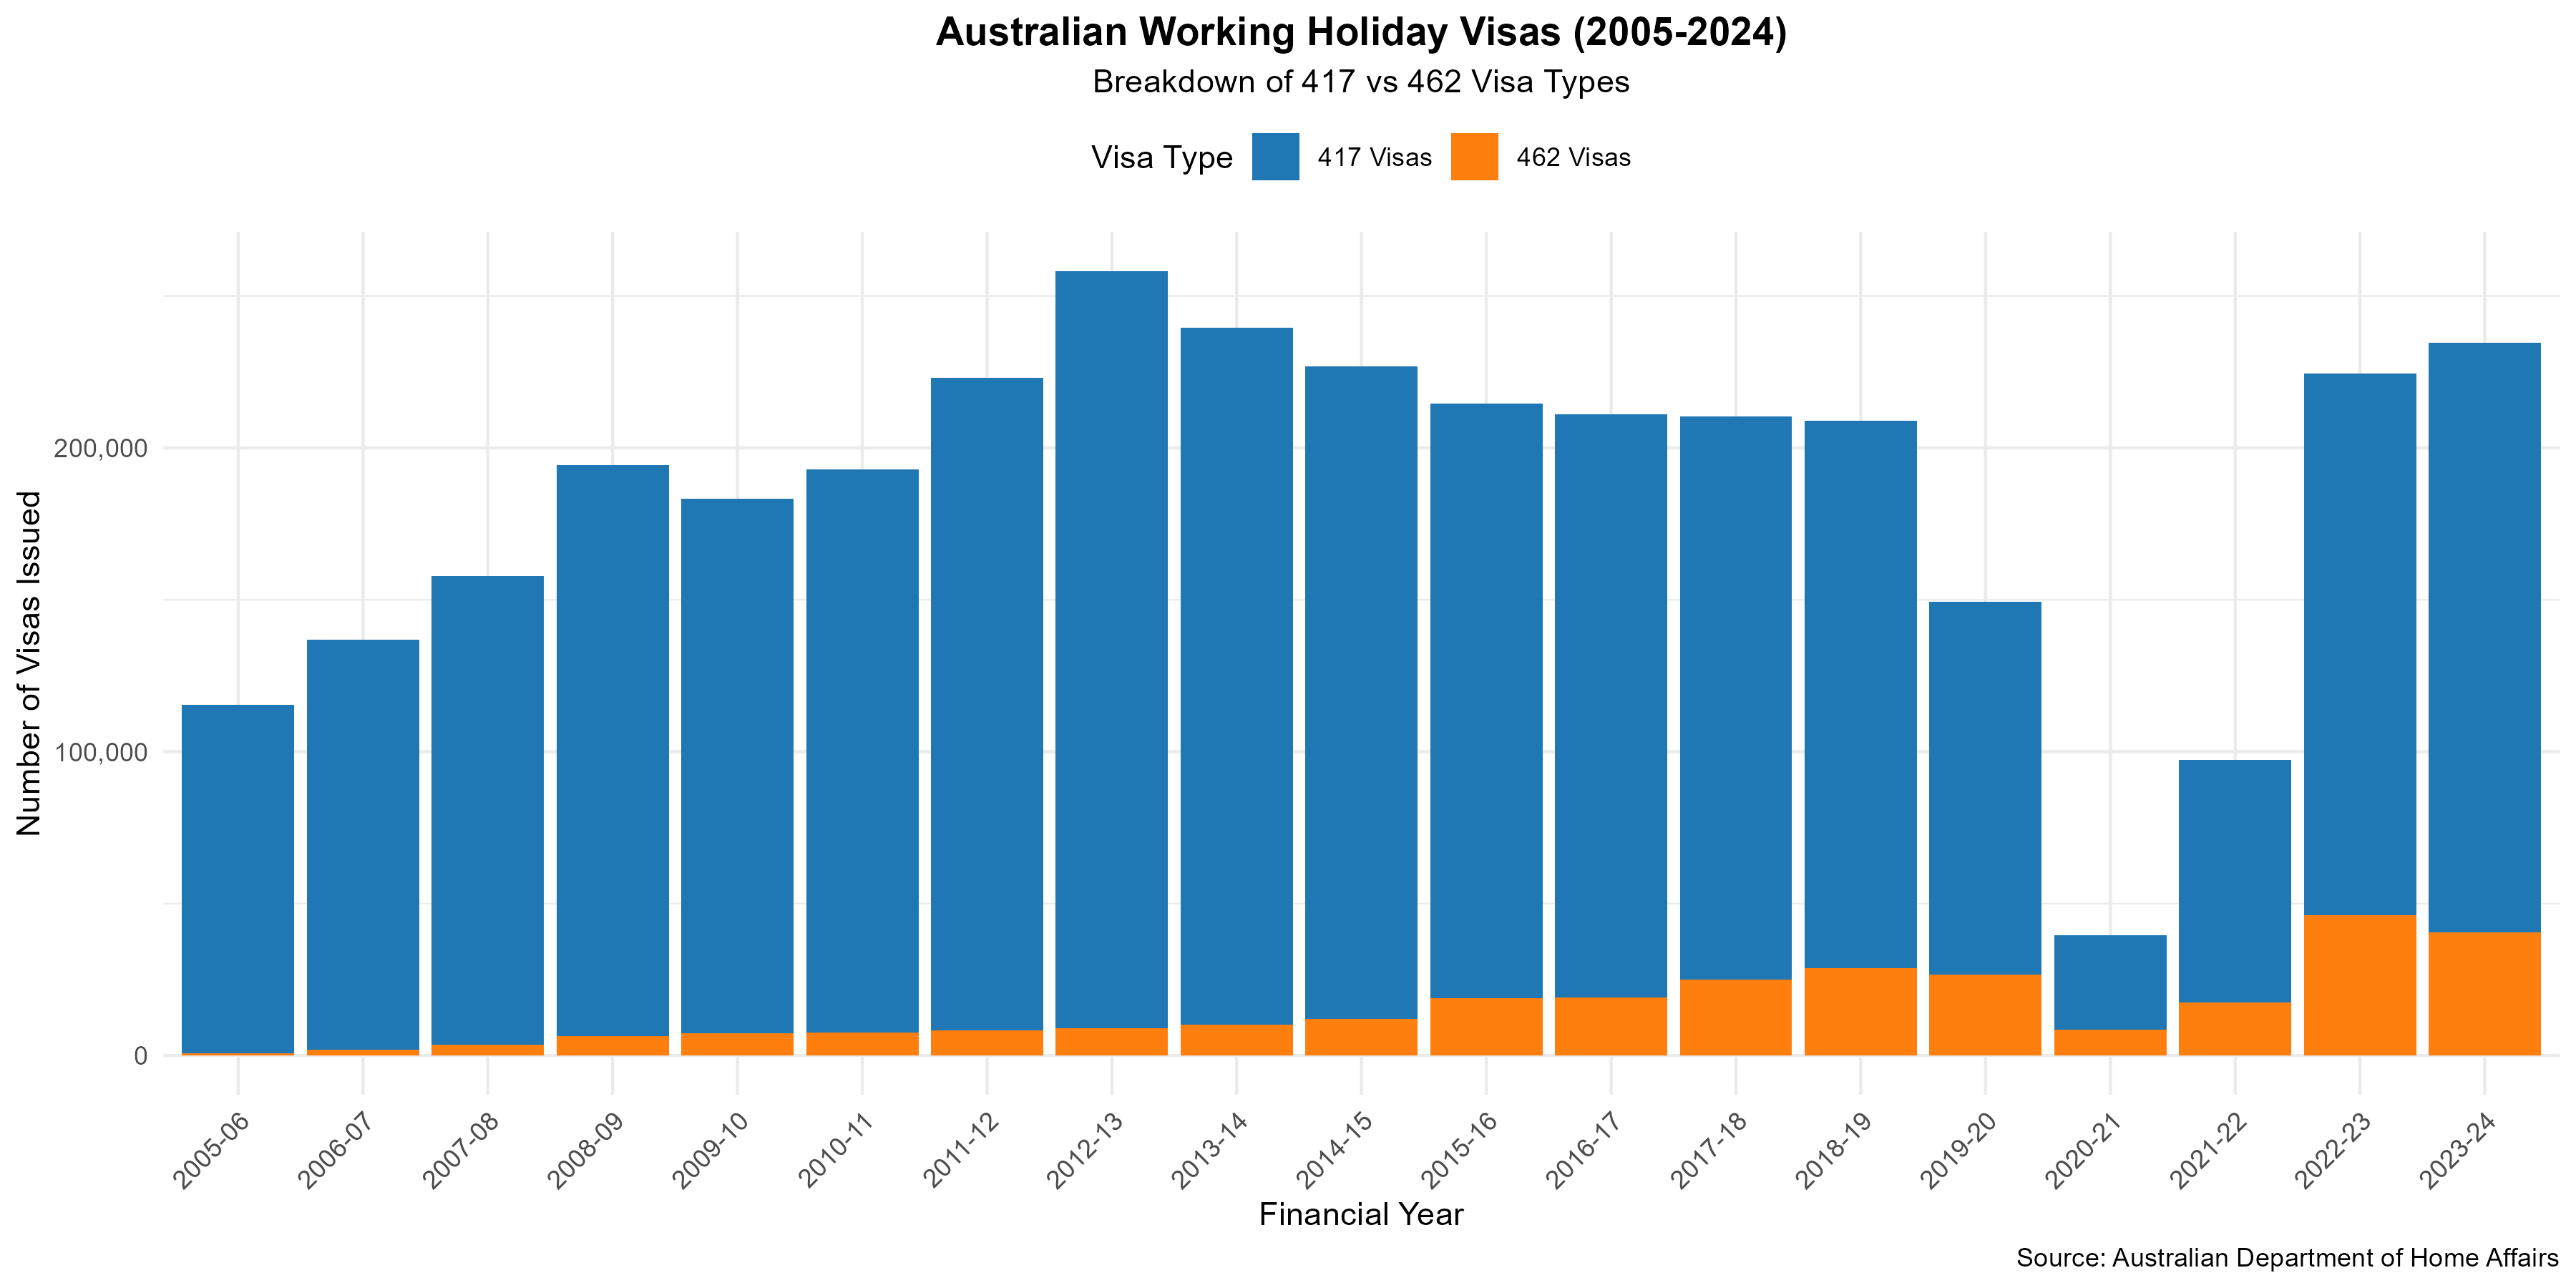
\includegraphics[width=0.9\columnwidth]{figures/australia_working_holiday_visas.png}
    %		\caption{Backpackers \cite{Curtain}}
    %%	\end{figure}



The increase in backpacker numbers has been substantial. From a pre-COVID average of 140,298 backpackers in Australia between June 2017 and December 2019, the number of WHM visa holders has reached an average of 180,000 over the four quarters to the end of September 2024. By the end of November 2024, the total number of WHM visas holders in Australia had jumped to as many as 213,394.    
%\subsection{Misuse of scheme}

\subsection*{Implications for Tonga's seasonal work}

The decline in Tonga’s participation in Australia’s PALM scheme—despite the program’s overall growth— highlights critical vulnerabilities in Tongas labor scheme future. The shift toward more strict employment regulations (i.e guaranteed hours, improved worker protections) has inadvertently made short-term contracts less attractive to employers, who now favor backpackers to offset compliance costs. For Tonga, where 67\% of PALM workers rely on short-term roles, this trend threatens a key source of remittances and exposes the economy to two risks: \\ \textbf{(1)} reduced income stability for households dependent on seasonal work, and \\ \textbf{(2)} weaker bargaining power as employers pivot to cheaper, more flexible labor sources like working holidaymakers. \\

While the reforms address exploitation, Tonga must urgently diversify its labor export strategies—by upskilling workers for long-term contracts or developing domestic alternatives—to avoid being sidelined in a competitive mobility landscape. The data underscores a harsh reality: without adaptation, Tonga’s seasonal work sector risks becoming collateral damage in host countries’ labor market adjustments.

\newpage

\newpage

\section{Recognized Seasonal Employer (RSE)}

   %https://www.immigration.govt.nz/assets/inz/documents/statistics/statistics-rse-arrivals.pdf

   %uSE MACRO MODEL TO FORECAST IF WE STOPPED THE SCHEME
   %Skill mismatch ***
   %TVET upskill for skill match with overseas work
		
    \begin{tauenv}[frametitle=Background]
    By 2024, RSE reached a milestone of cumulating an aggregate of 50,000 workers since July 2007. The scheme has been transformative for New Zealand's economy whereby generating NZD \$7 billion in annual export earnings for the horticulture and viticulture industry - the ranking this industry the $4^{th}$ largest export industry in New Zealand. Its success leading to the Government aim to reach an industry revenue of 12 billion by 2035.        
\end{tauenv}
		
        In contrast to PALM, the RSE scheme depicts a positive trend, where the headline figures show Tonga's seasonal workers have been rising relatively post-covid from 987 in 2022 to 1307 in 2024.
        


        	\begin{figure}[H]
    		\centering
    		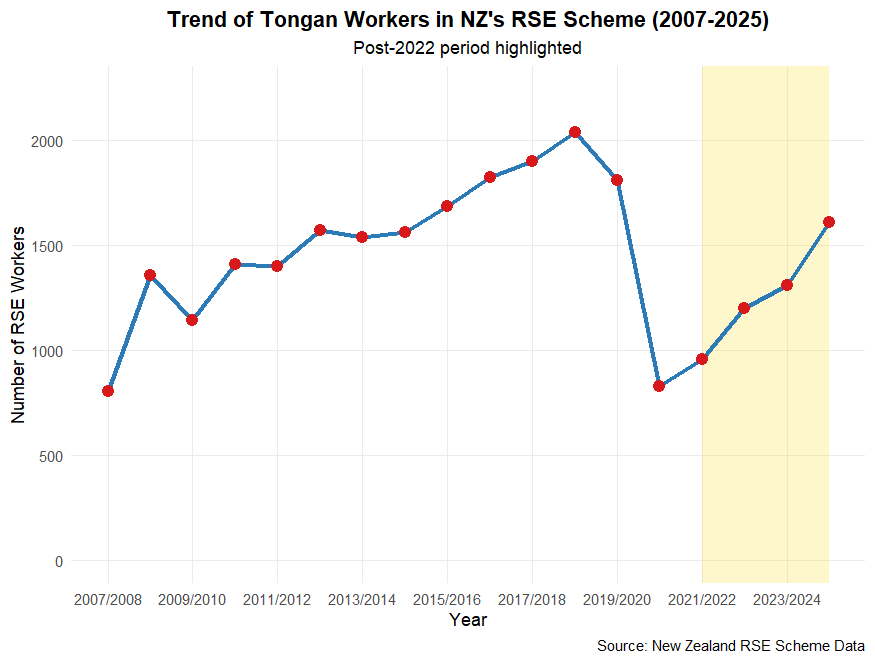
\includegraphics[width=0.9\columnwidth]{figures/RSE_scheme.png}
    		\caption{Post Deed of Agreement favors long-term contracts}
    		\label{fig:RSE}
    	\end{figure}



        In conjunction with Tonga's decline in ST PALM roles, the RSE scheme benefits from this. There is less direct competition from Australia's seasonal scheme at the enterprise level. Tonga's HIES (2021) indicated a number Tongans experimented with the short-term role employments for both schemes, yet no major shift has realized between the worker numbers from one scheme to another. Moreover, major source countries: Vanuatu, Samoa, and Tonga gave serious scrutiny towards aspects of participating in the NZ scheme (for reasons of exploitation and social issues arising from the scheme), yet RSE's recruitment numbers are growing steadily and meeting their output and productivity goals. Following the steady growth of RSE's worker count and productivity, their reports provide insightful surveys that can inform our policy directions. 

\textbf{Insights from RSE worker productivity}

	\begin{figure}[H]
    		\centering
    		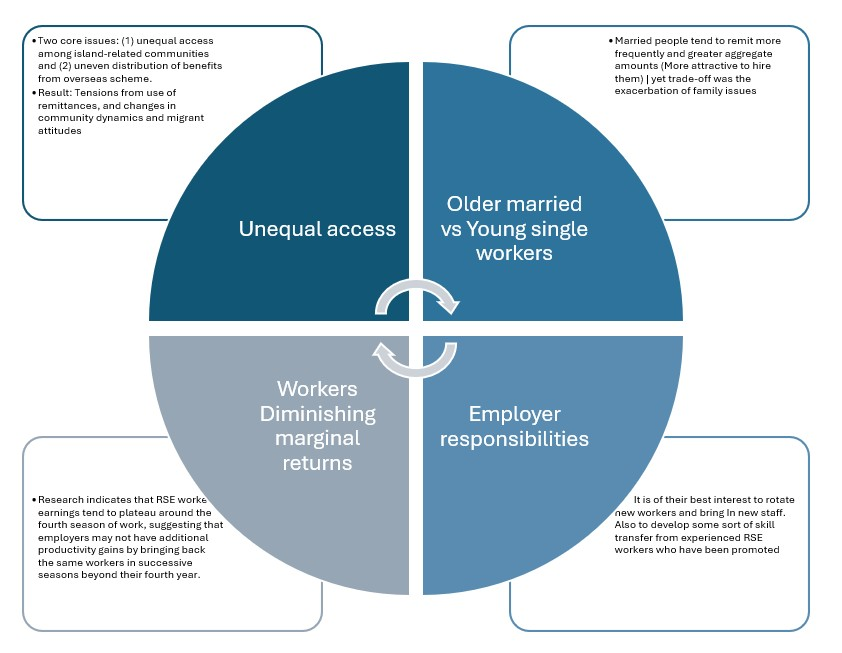
\includegraphics[width=0.75\columnwidth]{figures/Insights_RSE.jpg}
    		\caption{Productivity insights}
    		\label{fig:backpacker}
    	\end{figure}



        According to Bredford (2017), the vision of the RSE program was to make \textit{selective} use of the scheme to help families from the pacific earn income and better their livelihoods, so policies targeted aspects of workers settling in and restrictions around bringing family so they would not necessarily want to return to New Zealand year after year. Yet the interest to come back and work over succcessive seasons leads to questions around the inequity of access to the scheme as well as an overdependence on a scheme that may not always be available. The following insights are developed to inform preparing seasonal workers for the skills necessary to further their livelihoods back in the islands:

\begin{itemize}
        \item \textbf{Unequal Access to the scheme}: The selection process is varied across PICs. Tonga seems to be performing well under this metric - employing  a village-level nomination of people for RSE targetting those from relatively poor households. In contrast, Vanuatu tends to selects workers from wealthier than average households, whilst PNG and Fiji give the recruitment power to community leaders and government heads.
        
        
        % While from a development perspective spreading opportunities to participate in seasonal work is important, there are potential trade-offs between spatial equity and efficiency as employers may seek to minimise their costs by recruiting workers from the most convenient locations.

       \item \textbf{Older/Younger or Single/Married?} - Findings from the RSE Remittance Pilot Project show that older workers and those who are married tend to remit more frequently, and send home larger aggregate amounts, than younger workers and those who are single. Therefore, if remittances are considered the primary gain from participation in seasonal work, it makes sense for employers to recruit older, married workers. However, research on the Canadian Seasonal Agricultural Workers Program (SAWP)has found that employers’ preference for older workers with children and/or other dependents exacerbates negative impacts on families, illustrating there can be trade-offs between the financial gains and social costs for migrant households     

    \item \textbf{Diminishing marginal return} - Research indicates that RSE workers’ earnings tend to plateau around the fourth season of work, suggesting that employers may not have additional productivity gains by bringing back the same workers in successive seasons beyond their fourth year.



    \item \textbf{Employer responsibilities} - Noting the above, alot of the solution lies with the employers. It is of their best interest to rotate new workers and bring In new staff. Also to develop some sort of skill transfer from experienced RSE workers who have been promoted




        \end{itemize}
         
         
         
         \subsection*{Implications for Tonga's seasonal work}
         
        In summary, the decline in Australia’s ST PALM roles and so Tonga’s reliance on RSE raises long-term concerns and provides insight into the aspects that inform good policy. The above insights concerning the worker productivity traits, period of effectiveness, equitable distribution of seasonal work, and the emphasis on the role of employers in rotating workers are important elements to consider.
        
        
        
        
        %While Tonga’s village-based recruitment helps target poorer households  inequities persist, such as older, married workers remitting more but facing social costs from prolonged absences. Productivity plateaus after four seasons suggest diminishing returns for both workers and employers, highlighting the need for skill-transfer programs and rotational policies to prevent dependency. For Tonga, maximizing gains while mitigating risks requires balancing RSE’s short-term income opportunities with investments in local livelihoods to reduce vulnerability to external labor market shifts.
         
         
         
         
         
         %offering insights into worker productivity and equitable distribution. Reports indicate that Tongan workers under RSE often achieve higher productivity metrics compared to other Pacific nations, attributed to targeted skills training and cultural familiarity with NZ’s agricultural sector. Additionally, the program has made strides in equitable worker distribution, ensuring broader regional participation across Tonga rather than concentrating benefits in urban centers. This contrast highlights RSE’s relative success in balancing employer needs with sustainable opportunities for Tongan laborers, even as PALM’s short-term roles diminish. However, questions remain about whether RSE’s model can scale to offset PALM’s losses, particularly for workers reliant on Australia’s higher wages.
 


\section{Policy}
\subsection{Existing policies}

To date, a Tongan labor mobility supply exists that is "equitable, inclusive, can broaden the range of appropriate and aligned skills for both domestic and international supply." The contents are not disclosed online or by MTED (pout) .......

\noindent Yet a final consideration must be made of the existing policies in other PIC that could inform Tonga's policy reform 

\begin{itemize}
\item \textbf{Samoa's Labor Mobility Policy} - In 2023, Samoa's government approved a new labor mobility policy that targetted two key areas: 
\begin{enumerate}
    \item Addressing Inequity - Aspects of this policy prioritized the mobilisation of unemployed people, especially those who have gone without employment for 6 months or more. Other efforts targeted the equal distributions of opportunity through these schemes by utilizing the newly established Constituency Committees that would prioritize offerring the mobility programs to rural villages.
    \item Mitigating Exploitation - The elements of this theme targetted the safety measures for workers who were deployed overseas. For one, all approved employers wishing to recruit from Samoa had to first inform the Government (MCIL-LEEP) of its intentions. Higher transparency was expected from private recruiters to monitor the recruitment process and avoid unethical practises where workers bear the up-front costs or recruitment frees.
\end{enumerate}


\item \textbf{Vanuatu's Labor Mobility Policy} - The Vanuatu Government launched its Labour Mobility Policy for 2024-2027 in response to the evolving challenges coming from seasonal work programmes (particularly, family disruptions from long abscences). This targetted five key areas:
\begin{enumerate}
    \item Legislative and Institutional Reform - improving regulations to better manage labor mobility and provide stronger protection for workers.
    \item Data collection and systems coordination - Strengthen accountability and data collection systems for better informed decision making.
    \item Labor mobility support management and reintegration strategies - Promoting decent work, skills transfer and reintegration returning workers back into the source country job market.
    \item Child-centred Family and Community Social Protection - Support the welfare of children and families affected by labour mobility.
    \item Worker Welfare and Benefits - Advocating for better working conditions and contract terms for Vanuatu workers.
\end{enumerate}

\end{itemize}

The policy responses from Samoa and Vanuatu are strongly relevant to Tonga's position given that the issues they are addressing are the same issues Tonga is facing.


\subsection{Tonga's policy}

\begin{tauenv}[frametitle=Policy Response]
        From the above analysis of PALM, RSE, and the existing policies from Samoa and Vanuatu, the following gaps are identified with Tonga's labor mobility scheme:  
        \begin{itemize}
            \item The need to upskill workers in Tonga for more Long-Term roles (learning from PALMs deed revision)
            \item Reintegration strategies that help returning workers transition back into the island economy (Learning from NZ insights on worker rotation)
            \item Long term educational planning for improved alignment of skills (Learning from 
            \item Higher transparency and better coordination between Tonga government and seasonal employers
            \item Improve data collection systems for better informed decision making processes (Learning from vanuatu's LMS)
            \item Support for families affected by labor mobility parental abscences (Learning from WCCC)

        \end{itemize}
\end{tauenv}

[Detailed writing of the above points \^]
%\newpage

\section{Annex}

	
    	\begin{figure}[H]
    		\centering
    		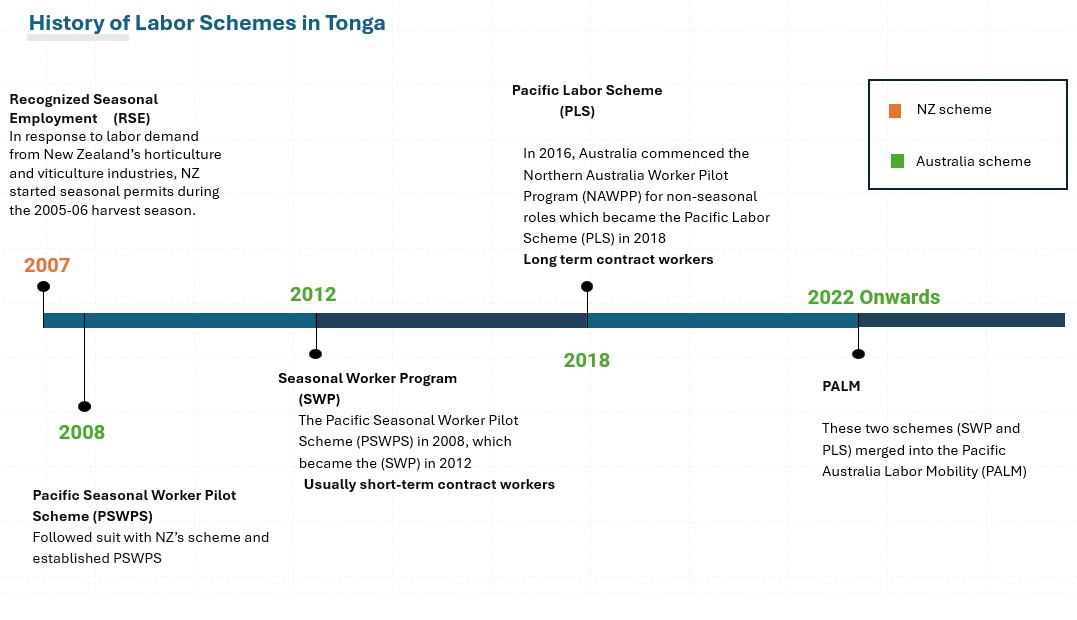
\includegraphics[width=0.9\columnwidth]{figures/timeline_LS.jpg}
    		\caption{History of Labor Schemes in Tonga}
    		\label{fig:Timeline}
    	\end{figure}


\begin{table}[htbp]
\centering
\caption{RSE and PALM participants by financial year}
\label{tab:rse-palm}
\begin{tabular}{lrr}
\toprule
\textbf{Financial year} & \textbf{RSE} & \textbf{PALM} \\
\midrule
2012/13 & 1573 & 1199 \\
2013/14 & 1600 & 1497 \\
2014/15 & 1563 & 2179 \\
2015/16 & 1687 & 2624 \\
2016/17 & 1899 & 2690 \\
2017/18 & 2790 & 2790 \\
2018/19 & 3738 & 3738 \\
2019/20 & 2025 & 2025 \\
2020/21 &  826 &  746 \\
2021/22 &  957 & 6035 \\
2022/23 & 1202 &  5320 \\
2023/24 & 1307 & 3040 \\
2024/25 & 1608 & 3480 \\
\bottomrule
\end{tabular}

\tabletext{Source: New Zealand Immigration \& PALM}
\end{table}
%\section{Econometric Model}

%\begin{equation} \label{ec:equation}
%	Remittances = \beta_0 + \beta_1 *PALM + \beta_2*RSE + \epsilon
%	\end{equation}

%\section{Overseas work life}

%It would be nice to have a section on important issues such as overstaying. As well as reports on the great successes of these programs as well but from the destination country rather than from Tonga's point of view

%\begin{table}[h]
%\centering
%\caption{PALM Program Participants and Their Impact}
%\label{tab:palm_participants}
%\begin{tabular}{>{\raggedright}p{3cm}>{\raggedright}p{3cm}>{\raggedright}p{3cm}>{\raggedright}p{3cm}}
%\toprule
%\textbf{Name} & \textbf{Background} & \textbf{Role/Experience} & \textbf{Impact} \\
%\midrule

%Sesa Metui & From Nukuleka, Tonga; joined PALM in 2022 & Worked at meat processing in Australia & Provides financial support to family; shows economic empowerment through PALM \\

%\addlinespace[0.3cm]
%Ofa Ulupano & Transitioned from hospitality to horticulture & Leads teams and trains staff on a large berry farm & Demonstrates career growth and skill development opportunities within PALM \\

%\addlinespace[0.3cm]
%Luke (Ninatoputapu) & Participant and speaker at PALM Workshop 2025 & Shared personal transformation experience & Highlights improved livelihoods and new opportunities for Tongan workers \\

%\bottomrule
%\end{tabular}
%\end{table}

%\begin{table}[t] % Use 'table*' for full-width tables in two-column docs
%\centering
%\caption{PALM Program Participants (Simplified)}
%\label{tab:palm_simplified}
%\begin{tabular}{>{\raggedright}p{2.5cm}>{\raggedright}p{4cm}>{\raggedright}p{4cm}}
%\toprule
%\textbf{Name} & \textbf{Role/Experience} & \textbf{Impact} \\
%\midrule
%Sesa Metui    & Worked at meat processing in Australia           & Provides financial support to family; economic empowerment through PALM \\
%\addlinespace[0.2cm]
%Ofa Ulupano   & Leads teams and trains staff on a large berry farm & Demonstrates career growth and skill development within PALM \\
%\addlinespace[0.2cm]
%Luke (Ninatoputapu) & Shared personal transformation experience      & Highlights improved livelihoods for Tongan workers \\
%\bottomrule
%\end{tabular}
%\end{table}



%\section{Recommendation}


%\section{Contact}
    
 %   \noindent\faEnvelope[regular]\hspace{7pt}amoeaki@finance.gov.to  \\
  %  \faInstagram\hspace{8pt}neyo\_02



%----------------------------------------------------------

\printbibliography

%----------------------------------------------------------

\end{document}